\documentclass[11pt, a4paper, twocolumn]{article}


% --- Paquetes de Idioma y Codificación ---
\usepackage[utf8]{inputenc}
\usepackage[spanish, es-nodecimaldot]{babel} % Configurado para español
\usepackage[T1]{fontenc}

% --- Tipografía y Estética ---
\usepackage{mathpazo} % Fuente Palatino, elegante y legible
\usepackage{microtype} % Mejora el espaciado entre letras y palabras

% --- Geometría de Página ---
\usepackage[margin=2.5cm, top=3.8cm, headheight=65pt, headsep=0.8cm]{geometry}
\columnsep 0.6cm % Espacio entre columnas
\usepackage{float}

% --- Matemáticas Avanzadas ---
\usepackage{amsmath, amsfonts, amssymb, amsthm}
\usepackage{mathtools}

% --- Gráficos y Tablas ---
\usepackage{graphicx}
\usepackage{booktabs} % Para tablas con estilo profesional (sin líneas verticales)
\usepackage{caption}
\captionsetup{labelfont=bf, font=small} % Captions en negrita y pequeñas

% --- Hipervínculos y Referencias ---
\usepackage[colorlinks=true, allcolors=blue]{hyperref}
\usepackage[capitalize]{cleveref} % Referencias inteligentes (ej: Fig. 1)
\usepackage{biblatex}
\addbibresource{polarizacion.bib}

% --- Título y Autores ---
\title{\textbf{\Large Polarización}}
\author{
    \textbf{Truchado Iniesta, Eduardo}, \textbf{Sanz Rubio, Juan} \\
    \small Grado de Física, UCLM. \texttt{juan.sanz1@alu.uclm.es} \\
    \small Grado de Física, UCLM. \texttt{eduardo.truchado@alu.uclm.es}
}
\date{\small 2 Marzo 2026}


\usepackage{fancyhdr}
%\usepackage{graphicx}

% --- Configuración del Encabezado ---
\pagestyle{fancy}
\fancyhf{} % Limpia encabezado y pie de página
\renewcommand{\headrulewidth}{0.4pt} % Línea horizontal bajo el encabezado

% Imagen a la IZQUIERDA
\fancyhead[L]{
\includegraphics[height=2cm]{logoFCTo.png}}

\fancyfoot[C]{\thepage}


\fancypagestyle{plain}{
    \fancyhf{} % Limpia el estilo plain por defecto
    \fancyhead[L]{
\includegraphics[height=2cm]{logoFCTo.png}} % Mantiene tu logo
    \fancyfoot[C]{\thepage} % Fuerza el número de página
    \renewcommand{\headrulewidth}{0.4pt} % Mantiene la línea
}

% --- Inicio del Documento ---

\begin{document}

\maketitle
\thispagestyle{fancy}

%Resumen

\begin{abstract}
En esta práctica se han realizado diferentes montajes relacionados con la polarización para analizar diferentes fenómenos: 

\begin{enumerate}
    \item \textbf{Ecuaciones de Fresnel y ángulo de Brewster:} Mediante el estudio de la reflexión de un láser a través de un
    prisma, obtendremos el ángulo de Brewster y el índice de refracción del prisma.
    \item \textbf{Ley de Malus:} Mediante un analizador de intensidad y un polarizador que nos permite variar el ángulo, buscamos
    mostrar la ley de intensidades de Malus.
    \item \textbf{Cálculo del vector de Stokes:} Montaremos diferentes sistemas con polarizadores y láminas para ver como varían los vectores de Stokes.
    \item \textbf{Birrefringencia:} Vemos cualitativamente como afectan los materiales birrefringentes a un sistema lumínico de un láser.
\end{enumerate}

\end{abstract}

\section{Introducción}

La polarización es una propiedad intrínseca de las ondas electromagnéticas, esta puede estudiarse mediante diferentes métodos. En nuestro utilizaremos diferentes medios ópticos para
estudiar el comportamiento de la luz, en este caso un láser con $\lambda = 635 nm$, al pasar por ellos.

\begin{itemize}
    \item La luz refracta con un cierto ángulo cuando sufre un cambio de medios con diferente índice de refracción. Un caso interesante es aquel donde se cumple la relación de Brewster $tan(\theta_{B}) = \frac{n'}{n}$ donde $\theta_{B}$ es el ángulo de Brewster que es aquel donde no hay reflexión.
    \item Por otro lado la intensidad de la luz también varía al cambiar su ángulo de polarización, esta variabilidad sigue una ley conocida como ley de Malus, $I(\theta) = I_{0}cos^2(\theta)$.
    \item Además los sistemas polarizados pueden describirse perfectamente a través de un vector denominado "vector de Stokes", que tiene la siguiente forma, $\vec{S} = (S_{0}, S_{1}, S_{2}, S_{3})^{T}$. 
    
\end{itemize}

\section{Objetivos}
Los objetivos son familiarizarse con procedimientos ópticos utilizados para el estudio de diferentes fenómenos ópticos asociados a la polarización. 
\section{Metodología}

Para los procedimientos aquí propuestos se han utilizado en todos un láser de luz roja con $\lambda = 630 nm$ y un fotómetro de thorlabs \cite{thorlabs_opm}. Ahora el montaje para cada procedimiento es diferente. 

\subsection{Ecuaciones de fresnel y ángulo de Brewster}

\begin{figure}[H]
    \centering
    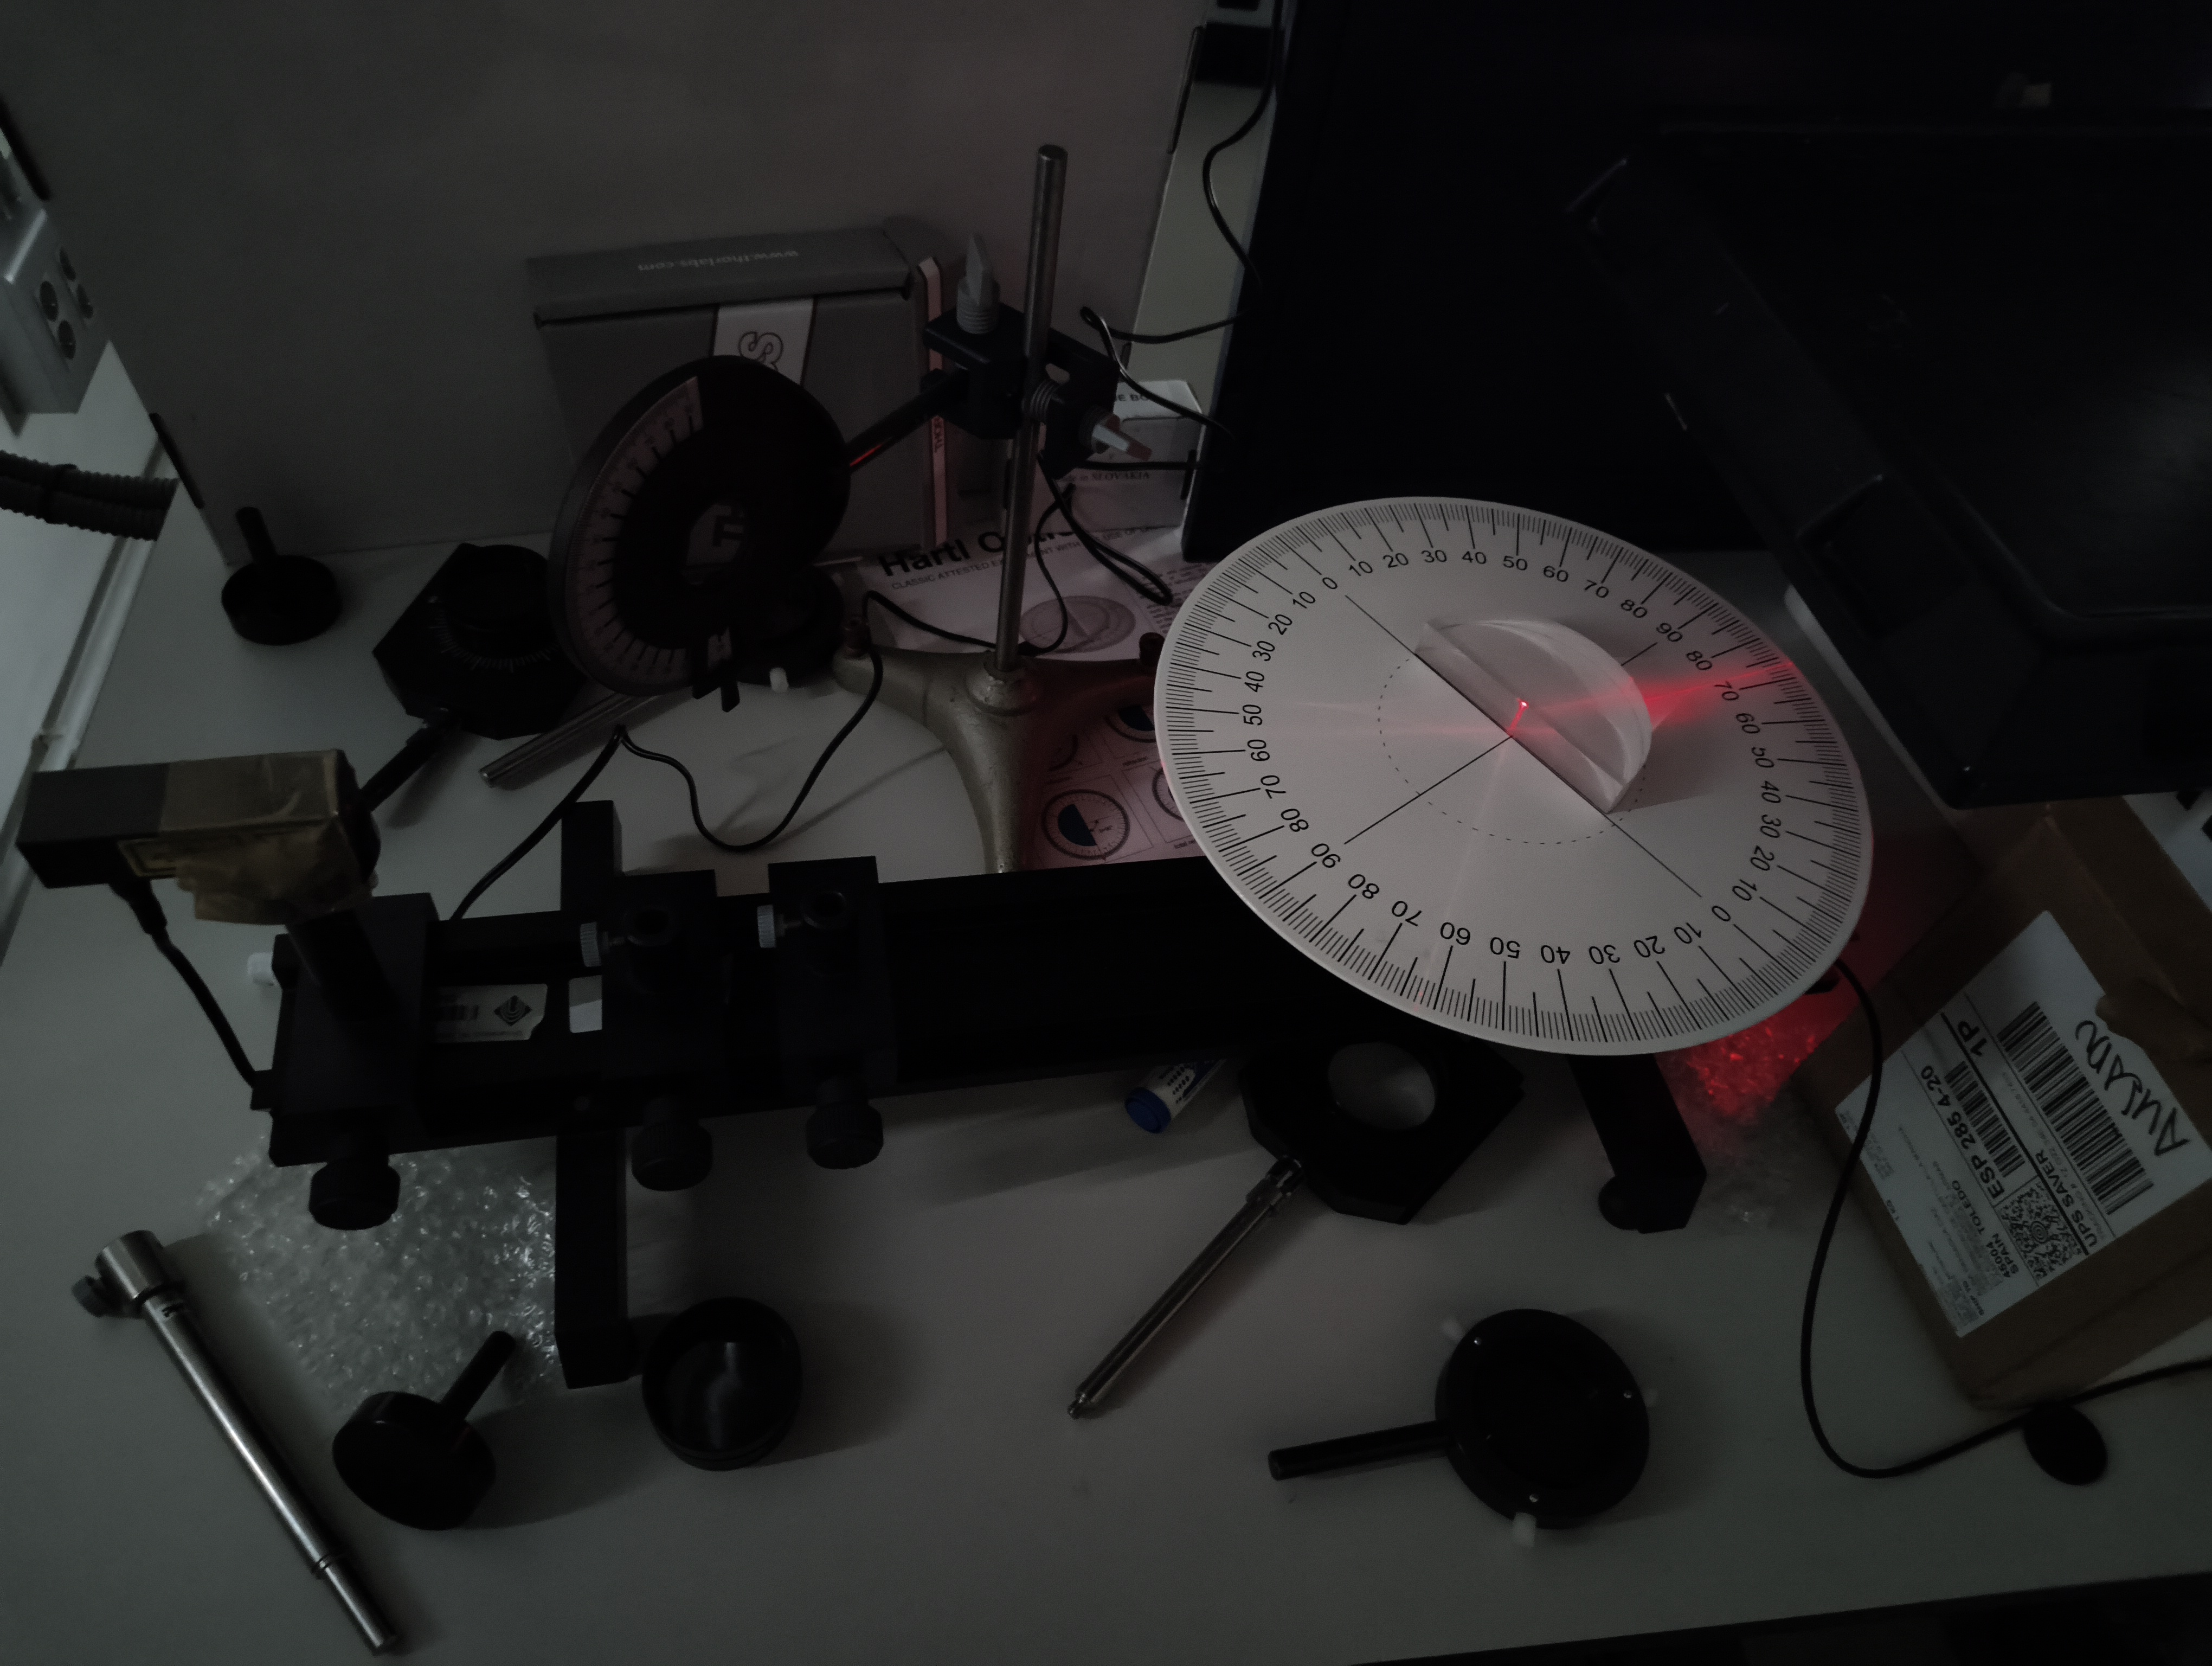
\includegraphics[width=0.4\textwidth]{fotos_practica/montaje_brewster.jpg}
\end{figure}

En este caso se ha colocado el prisma en un goniómetro calibrado que nos permitirá medir el ángulo para diferentes casos. La luz saliente del láser está polarizada linealmente inicialmente, luego procederemos a colocar
un polarizador que nos ayude a que la luz pase a ser perpendicularmente polarizada. 

Con los datos de ángulos representaremos $I$ frente a $\theta$ y donde se encurntre el mínimo de la curva, tendremos el ángulo de Brewster. Con ello usando la relación $tan(\theta_{B}) = \frac{n'}{n}$ podremos hallar
el índice de refracción del prisma.

\subsection{Ley de Malus}

\begin{figure}[H]
    \centering
    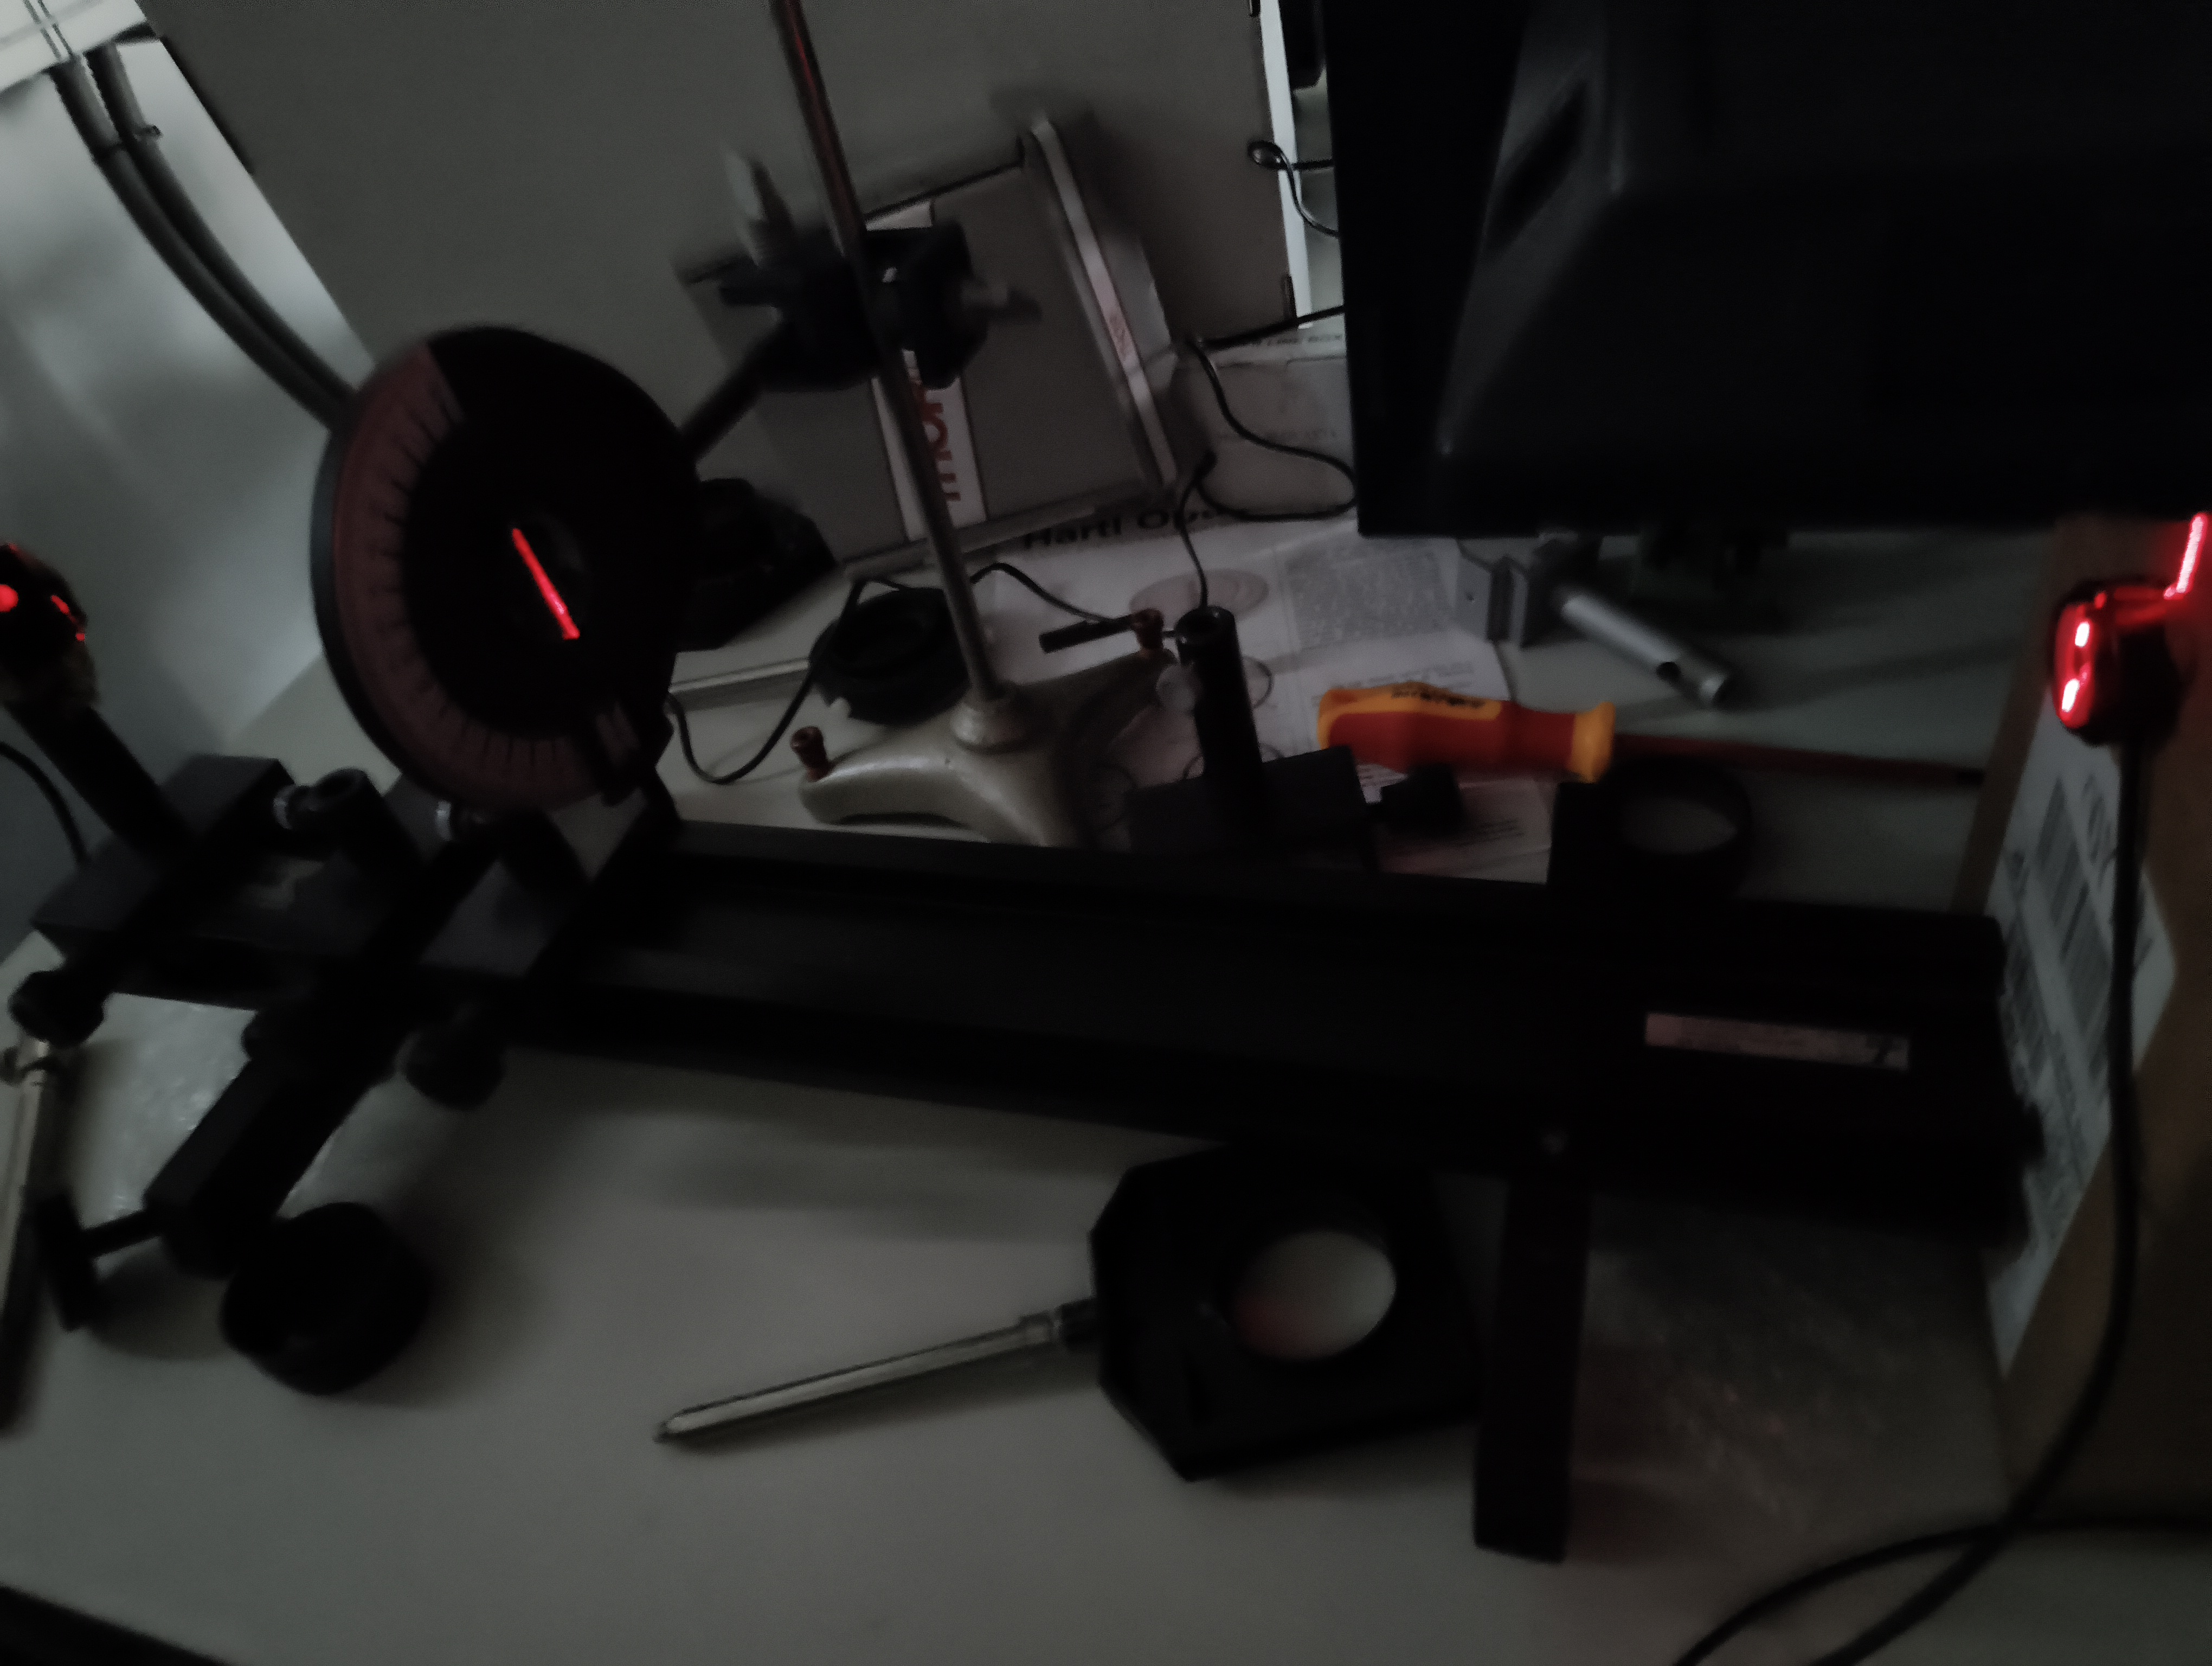
\includegraphics[width=0.4\textwidth]{fotos_practica/montaje_malus.jpg}
\end{figure}

Ahora se ha colocado un polarizador que nos permite variar el ángulo de polarización con un cierto margen de error. Con esto representaremos I frente a $\theta$ para verificar que la función obtenida es un $cos^{2}(\theta)$.

\subsection{Vector de Stokes}

\begin{figure}
    \centering
    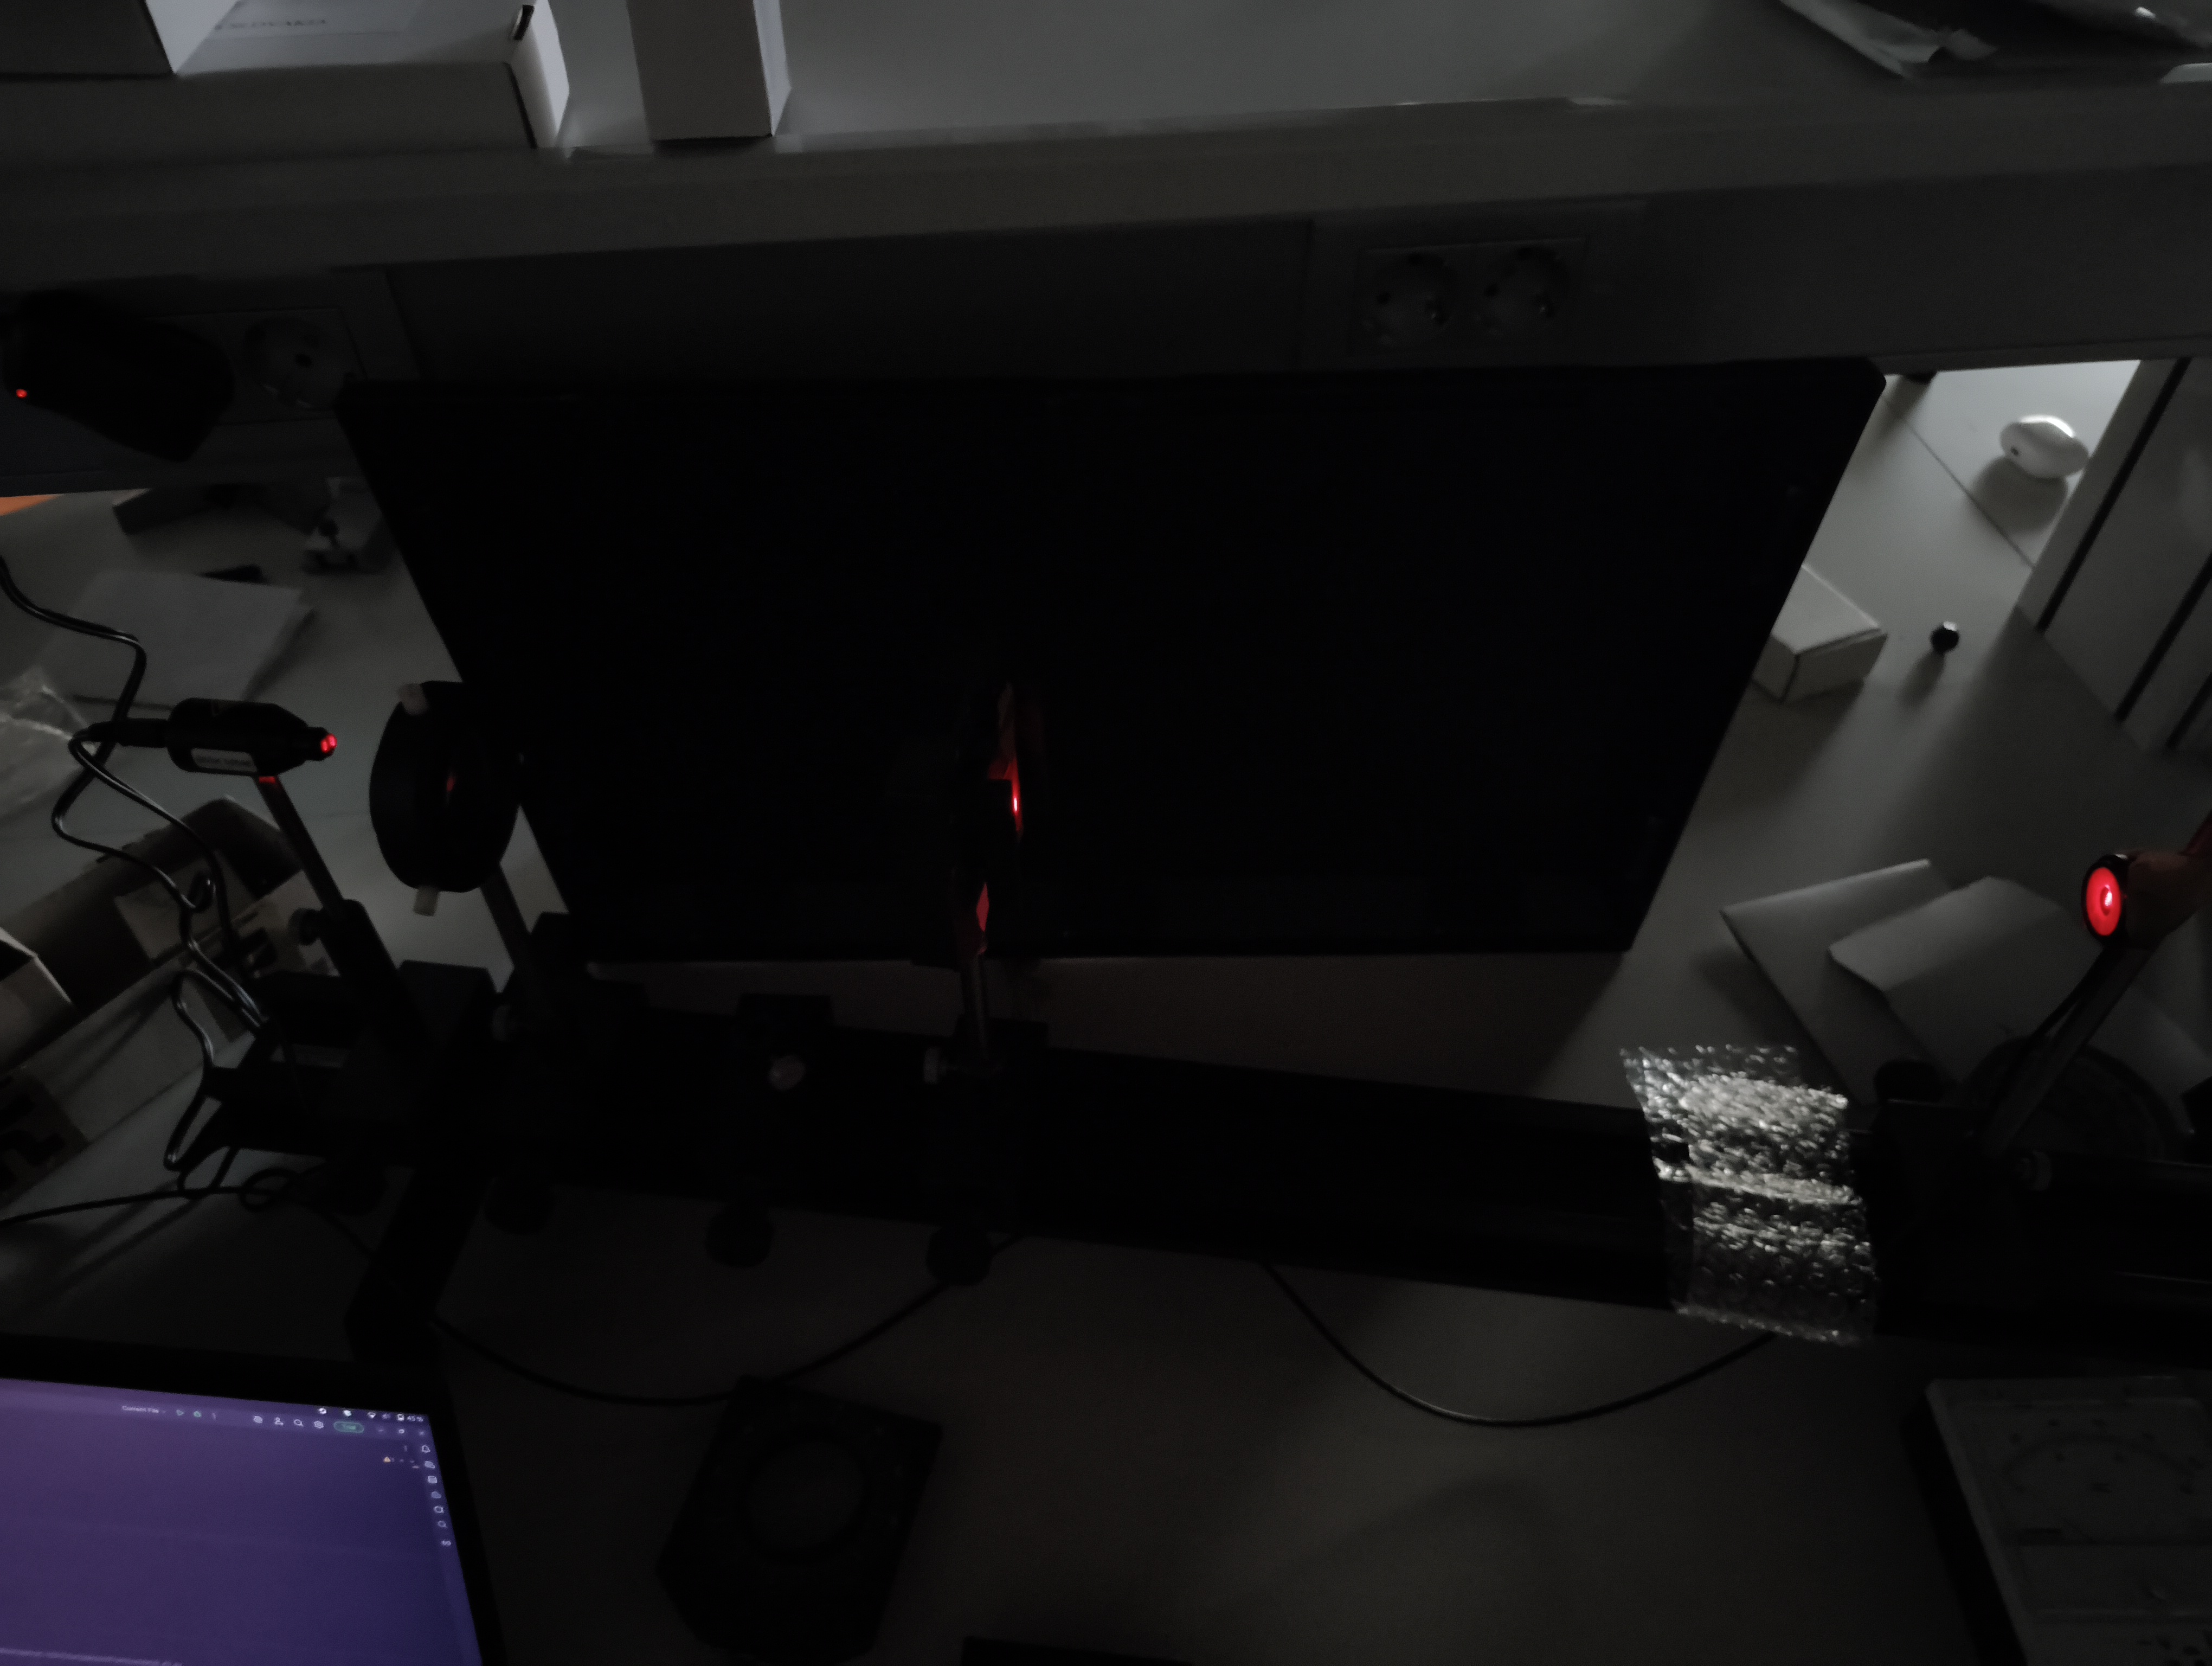
\includegraphics[width=0.4\textwidth]{fotos_practica/montaje_stokes.jpg}
\end{figure}

En este análisis se han ido montando diferentes sistemas conforme al orden pedido en la práctica. En este caso se ha realizado tanto para el caso A, luz lineal vertical, como para el caso B, luz circular.

\begin{enumerate}
    \item $I_{total}$ (sin analizador)
    \item $I_{v}$ (con analizaodr vertical a 90º)
    \item $I_{45}$ (con analizador a 45º)
    \item $I_{CD}$ (con analizador circular)
\end{enumerate}

Con estos se han calculado los vectores de Jones para cada caso y calculados con los valores teóricos $(1, -1, 0, 0)$ y $(1, 0, 0, 1)$ respectivamente. 
\newpage

\section{Tratamiento de datos}

A continuación mostraremos las tablas de datos obtenidos. Para cada parte.

\subsection{Ecuaciones de fresnel y ángulo de Brewster}

\begin{table}[H]
    \centering
    \small
    \begin{tabular}{cccc}
        \hline
        $\theta$ (º) &   $I$ (mw) & $\Delta \theta$ (º)   & $\Delta I$ (mw)   \\
        \hline
                            5 &     7.45 & $\pm 0.5$                    & $\pm 0.01$      \\
                            10 &     7.56 & $\pm 0.5$                    & $\pm 0.01$      \\
                            15 &     7.84 & $\pm 0.5$                    & $\pm 0.01$      \\
                            20 &     8.72 & $\pm 0.5$                    & $\pm 0.01$      \\
                            25 &     9.77 & $\pm 0.5$                    & $\pm 0.01$      \\
                            30 &    10    & $\pm 0.5$                    & $\pm 0.01$      \\
                            35 &    12    & $\pm 0.5$                    & $\pm 0.01$      \\
                            40 &    14    & $\pm 0.5$                    & $\pm 0.01$      \\
                            45 &    16    & $\pm 0.5$                    & $\pm 0.01$      \\
                            50 &    19    & $\pm 0.5$                    & $\pm 0.01$      \\
                            55 &    25    & $\pm 0.5$                    & $\pm 0.01$      \\
                            60 &    32    & $\pm 0.5$                    & $\pm 0.01$      \\
                            65 &    44    & $\pm 0.5$                    & $\pm 0.01$      \\
                            70 &    61    & $\pm 0.5$                    & $\pm 0.01$      \\
                            75 &    83    & $\pm 0.5$                    & $\pm 0.01$      \\
                            80 &   116    & $\pm 0.5$                    & $\pm 0.01$      \\
                            85 &   161    & $\pm 0.5$                    & $\pm 0.01$      \\
        \hline
    \end{tabular}
    \caption{Tabla de ángulos frente a intensidad normalizada para el caso vertical}
\end{table}


\begin{table}[H]
    \centering
    \small
    \begin{tabular}{cccc}
        \hline
        $\theta$ (º) &   $I$ (mw) & $\Delta \theta$ (º)   & $\Delta I$ (mw)   \\
        \hline
                            5 &     0.77 & $\pm 0.5$                    & $\pm 0.01$      \\
                            10 &     0.72 & $\pm 0.5$                    & $\pm 0.01$      \\
                            15 &     0.66 & $\pm 0.5$                    & $\pm 0.01$      \\
                            20 &     0.61 & $\pm 0.5$                    & $\pm 0.01$      \\
                            25 &     0.52 & $\pm 0.5$                    & $\pm 0.01$      \\
                            30 &     0.48 & $\pm 0.5$                    & $\pm 0.01$      \\
                            35 &     0.39 & $\pm 0.5$                    & $\pm 0.01$      \\
                            40 &     0.33 & $\pm 0.5$                    & $\pm 0.01$      \\
                            45 &     0.26 & $\pm 0.5$                    & $\pm 0.01$      \\
                            50 &     0.14 & $\pm 0.5$                    & $\pm 0.01$      \\
                            55 &     0.14 & $\pm 0.5$                    & $\pm 0.01$      \\
                            60 &     0.18 & $\pm 0.5$                    & $\pm 0.01$      \\
                            65 &     0.41 & $\pm 0.5$                    & $\pm 0.01$      \\
                            70 &     0.93 & $\pm 0.5$                    & $\pm 0.01$      \\
                            75 &     2.06 & $\pm 0.5$                    & $\pm 0.01$      \\
                            80 &     4.79 & $\pm 0.5$                    & $\pm 0.01$      \\
                            85 &     9.62 & $\pm 0.5$                    & $\pm 0.01$      \\
        \hline
    \end{tabular}
    \caption{Tabla de ángulos frente a intensidad normalizada para el caso perpendicular}
\end{table}

\vspace{0.3cm}

\subsection{Ley de Malus}

\begin{table}[H]
    \centering
    \small
    \begin{tabular}{cccc}
        \hline
        $\theta$ (º) &   $I$ (mw) & $\Delta \theta$ (º)   & $\Delta I$ (mw)   \\
        \hline
                    0 &     145    & $\pm 0.5$             & $\pm 0.01$        \\
                    5 &     143    & $\pm 0.5$             & $\pm 0.01$        \\
                    10 &     140    & $\pm 0.5$             & $\pm 0.01$        \\
                    15 &     133    & $\pm 0.5$             & $\pm 0.01$        \\
                    20 &     125    & $\pm 0.5$             & $\pm 0.01$        \\
                    25 &     115    & $\pm 0.5$             & $\pm 0.01$        \\
                    30 &     103    & $\pm 0.5$             & $\pm 0.01$        \\
                    35 &      89    & $\pm 0.5$             & $\pm 0.01$        \\
                    40 &      78    & $\pm 0.5$             & $\pm 0.01$        \\
                    45 &      67    & $\pm 0.5$             & $\pm 0.01$        \\
                    50 &      55    & $\pm 0.5$             & $\pm 0.01$        \\
                    55 &      44    & $\pm 0.5$             & $\pm 0.01$        \\
                    60 &      33    & $\pm 0.5$             & $\pm 0.01$        \\
                    65 &      23    & $\pm 0.5$             & $\pm 0.01$        \\
                    70 &      15    & $\pm 0.5$             & $\pm 0.01$        \\
                    75 &       9    & $\pm 0.5$             & $\pm 0.01$        \\
                    80 &       4.72 & $\pm 0.5$             & $\pm 0.01$        \\
                    85 &       2.66 & $\pm 0.5$             & $\pm 0.01$        \\
                    90 &       2.78 & $\pm 0.5$             & $\pm 0.01$        \\
                    95 &       5.1  & $\pm 0.5$             & $\pm 0.01$        \\
                    100 &       9.53 & $\pm 0.5$             & $\pm 0.01$        \\
                    105 &      16    & $\pm 0.5$             & $\pm 0.01$        \\
                    110 &      24    & $\pm 0.5$             & $\pm 0.01$        \\
                    115 &      34    & $\pm 0.5$             & $\pm 0.01$        \\
                    120 &      45    & $\pm 0.5$             & $\pm 0.01$        \\
                    125 &      57    & $\pm 0.5$             & $\pm 0.01$        \\
                    130 &      70    & $\pm 0.5$             & $\pm 0.01$        \\
                    135 &      82    & $\pm 0.5$             & $\pm 0.01$        \\
                    140 &      95    & $\pm 0.5$             & $\pm 0.01$        \\
                    145 &     107    & $\pm 0.5$             & $\pm 0.01$        \\
                    150 &     117    & $\pm 0.5$             & $\pm 0.01$        \\
                    160 &     127    & $\pm 0.5$             & $\pm 0.01$        \\
                    165 &     134    & $\pm 0.5$             & $\pm 0.01$        \\
                    170 &     135    & $\pm 0.5$             & $\pm 0.01$        \\
                    175 &     136    & $\pm 0.5$             & $\pm 0.01$        \\
                    180 &     136    & $\pm 0.5$             & $\pm 0.01$        \\
        \hline
    \end{tabular}
    \caption{Tabla de ángulos frente intensidad al variar la polarización con el polarizador}
\end{table}

\newpage
\subsection{Vector de stokes}

\begin{table}[h!]
\centering
\caption{Medidas de intensidad y Vector de Jones para el Caso A.}
\begin{tabular}{|l|c|}
\hline
\textbf{Estado de Medida} & \textbf{Intensidad $I$ (mW)} \\ \hline
Total ($I_{total}$) & $528.00 \pm 0.01$ \\ \hline
Vertical ($I_v$) & $352.00 \pm 0.01$ \\ \hline
Horizontal ($I_h$) & $0.74 \pm 0.01$ \\ \hline
A $-45^\circ$ ($I_{-45}$) & $167.00 \pm 0.01$ \\ \hline
A $+45^\circ$ ($I_{+45}$) & $191.00 \pm 0.01$ \\ \hline
Circular ($\lambda/4$) & $288.00 \pm 0.01$ \\ \hline
Circular ($-\lambda/4$) & $240.00 \pm 0.01$ \\ \hline
\end{tabular}
\end{table}


\begin{table}[h!]
\centering
\caption{Medidas de intensidad y Vector de Jones para el Caso B.}
\begin{tabular}{|l|c|}
\hline
\textbf{Estado de Medida} & \textbf{Intensidad $I$ (mW)} \\ \hline
Total ($I_{total}$) & $300.00 \pm 0.01$ \\ \hline
Vertical ($I_v$) & $104.00 \pm 0.01$ \\ \hline
Horizontal ($I_h$) & $103.00 \pm 0.01$ \\ \hline
A $-45^\circ$ ($I_{-45}$) & $200.00 \pm 0.01$ \\ \hline
A $+45^\circ$ ($I_{+45}$) & $163.00 \pm 0.01$ \\ \hline
Circular ($\lambda/4$) & $93.00 \pm 0.01$ \\ \hline
Circular ($-\lambda/4$) & $100.00 \pm 0.01$ \\ \hline
\end{tabular}
\end{table}

\vspace{0.5cm}


\section{Análisis de resultados}

\subsection{Ecuaciones de fresnel y ángulo de Brewster}
En este caso para hallar el ángulo de Brewster, 


\section{Conclusiones}

Tras el estudio podemos sacar ciertas conclusiones. En primer lugar, podemos observar que la dimensión fractal siendo esta cercana a $d\approx 2.5$
se encurntra en un punto medio entre las 2D y las 3D, lo que quiere decir que no es un objeto perfectamente plano o esférico, sino que su volumen no 
ocupa todo el espacio teniendo zonas con aire lo que hace variar su volumen general. 


En el caso de que hubieramos obtenido un valor experimental de $d = 3$, eso implicaría que la bola que hemos creado sería perfectamente esférica, 
lo que implicaría que estaríamos hablando de un objeto en 3D. 

\vspace{0.5cm}
Podemos sacar otras relaciones en base a la masa y el volumen como la densidad. Como $\rho = \frac{M}{V}$ y $V \propto R^d$, 
podemos decir que $\rho \propto D^{d-3}$. Y como $d < 3$, las bolas más grandes, con mayor masa serán menos densas que las más 
pequeñas y compactas. 

\vspace{0.5cm}

Otra relación interesante es la dependendia de $d$ con el tipo de material utilizado para formar las esferas y con el método (si han sido comprimidas o no). 
En nuestro caso podemos apreciar que el pael de aluminio es el que más se acerca a tener una dimensión igual a 3, mientras que el papel no comprimido se aleja más
si bien el comprimido tiene una dimensión mayor. Es decir cuanto más maleable o más se trabaje para asimilar a una esfera, mayor será la dimensión fractal obetnida.

\textbf{AQUÍ HABRÍA QUE COMPARAR EL ERROR OBTENIDO PARA m EXPERIMENTALMENTE CON EL OBTENIDO EN LA APLICACIÓN}

\vspace{1cm}
Para ver todo el análisis de datos realizado por los alumnos, se habilita este enlace al repositorio de github donde están todos los archivos de práctias: 

\section{Referencias}

\printbibliography

\end{document}